\begin{frame}[c]
    \frametitle{基于多孔硅可调谐光学滤光片的微光谱仪:概述}
    \begin{columns}
        \begin{column}{.6\textwidth}
            \begin{itemize}
                \item Lammel, G.;  Schweizer, S.; Renaud, P., Microspectrometer based on a \textcolor{purple}{tunable optical filter} of \textcolor{red}{porous silicon}. Sensors and Actuators A: Physical 2001, 92 (1), 52-59.
                \item \textcolor{blue}{重要性:}降低了工艺复杂度和成本。
                \item \textcolor{blue}{创新点:}\begin{itemize}
                          \item 通过改变滤波片的角度调节通带波长。
                          \item 采用多孔硅批处理技术,只需两个光刻步骤即可制作出可调谐滤光片。
                          \item 只需要使用一个探测器,降低了成本。
                      \end{itemize}
                \item \textcolor{blue}{意义:}消除了常见的增益变化和补偿问题。
            \end{itemize}
        \end{column}
        \begin{column}{.4\textwidth}
            \begin{figure}[!htb] %H为当前位置,!htb为忽略美学标准,htbp为浮动图形
                \centering %图片居中
                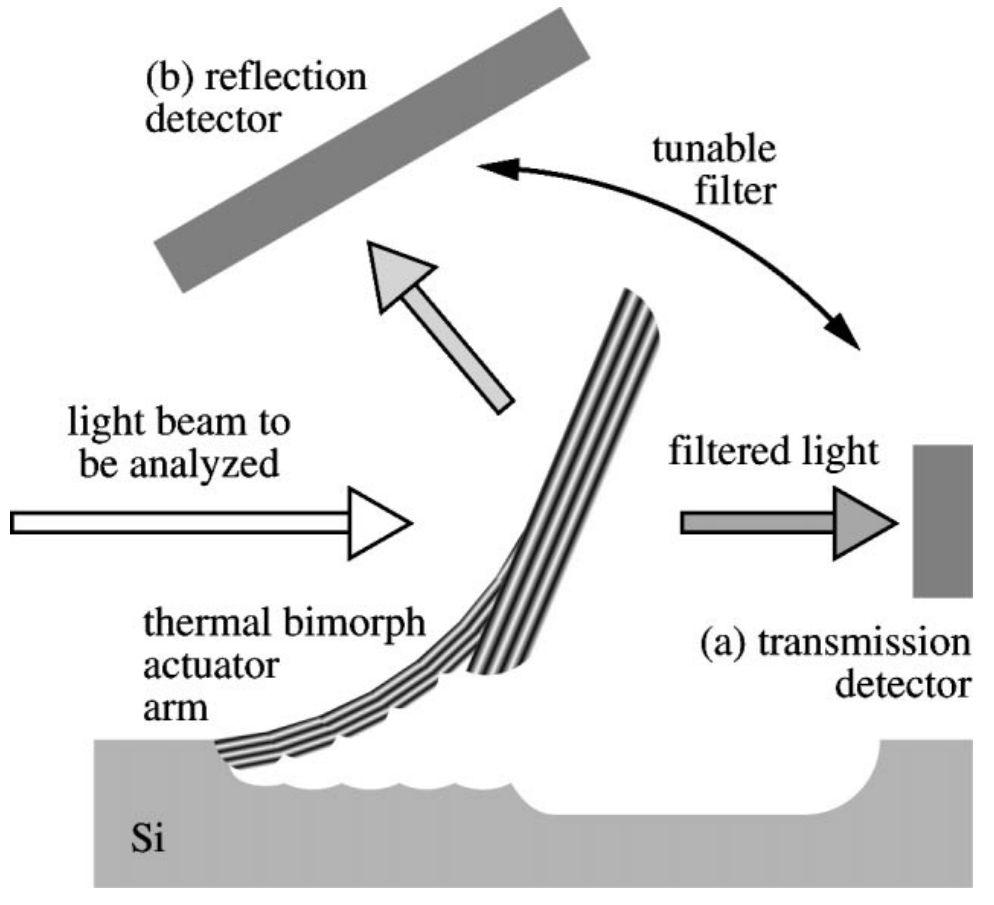
\includegraphics[width=1.\textwidth]{figures/Microspectrometer based on a tunable optical filter of porous silicon_1.png} %插入图片,[]中设置图片大小,{}中是图片文件名
                \caption{仪器结构示意图} %最终文档中希望显示的图片标题
            \end{figure}
        \end{column}
    \end{columns}

    \begin{figure}[!htb] %H为当前位置,!htb为忽略美学标准,htbp为浮动图形
        \centering %图片居中
        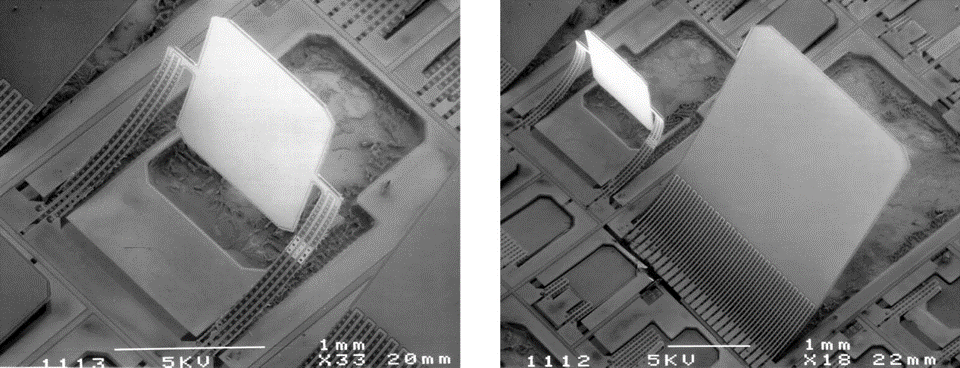
\includegraphics[width=.8\textwidth]{figures/Microspectrometer based on a tunable optical filter of porous silicon_2.png} %插入图片,[]中设置图片大小,{}中是图片文件名
        \caption{仪器结构示意图} %最终文档中希望显示的图片标题
    \end{figure}
\end{frame}

\begin{frame}[c]
    \frametitle{基于多孔硅可调谐光学滤光片的微光谱仪:原理和制造过程}
    \begin{description}
        \item[原理] 通过调节多孔硅的孔隙率可以改变其折射率,以此来制作反射镜形成法布里-珀罗滤光片。通过调节机械臂的角度改变光的入射角度,从而调节峰值波长。
    \end{description}

    工艺流程:
    \begin{itemize}
        \item $\mathrm{Si}_3\mathrm{N}_4$ 掩膜确定硅基底上多孔化和电抛光的区域
        \item 电化学刻蚀(氢氟酸和乙醇)形成多孔硅
        \item 电解抛光
        \item 在空气中晾干
        \item 充分氧化
    \end{itemize}

    \begin{columns}
        \begin{column}{.3\textwidth}
            \begin{figure}[!htb] %H为当前位置,!htb为忽略美学标准,htbp为浮动图形
                \centering %图片居中
                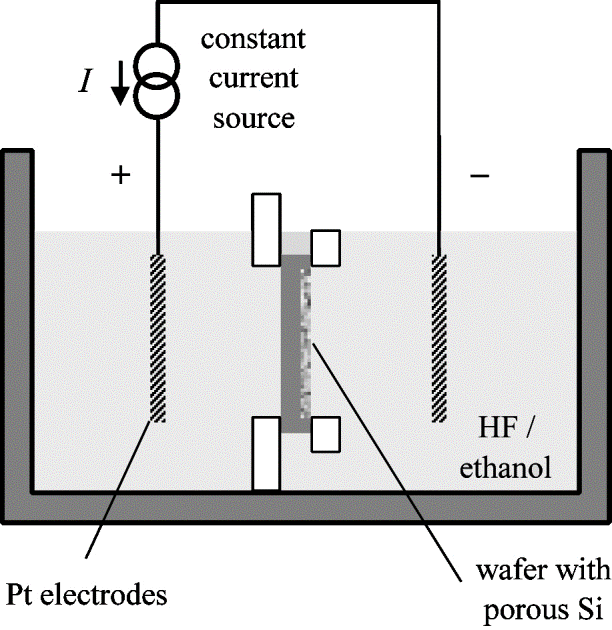
\includegraphics[width=1.\textwidth]{figures/Microspectrometer based on a tunable optical filter of porous silicon_5.png} %插入图片,[]中设置图片大小,{}中是图片文件名
                \caption{硅片多孔化和电解抛光的电化学腐蚀池} %最终文档中希望显示的图片标题
            \end{figure}
        \end{column}
        \begin{column}{.4\textwidth}
            \begin{figure}[!htb] %H为当前位置,!htb为忽略美学标准,htbp为浮动图形
                \centering %图片居中
                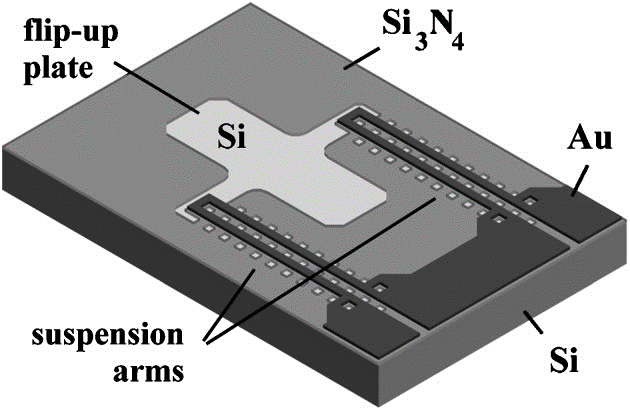
\includegraphics[width=1.\textwidth]{figures/Microspectrometer based on a tunable optical filter of porous silicon_6.png} %插入图片,[]中设置图片大小,{}中是图片文件名
                \caption{氮化硅掩膜} %最终文档中希望显示的图片标题
            \end{figure}
        \end{column}
        \begin{column}{.3\textwidth}
            \begin{figure}[!htb] %H为当前位置,!htb为忽略美学标准,htbp为浮动图形
                \centering %图片居中
                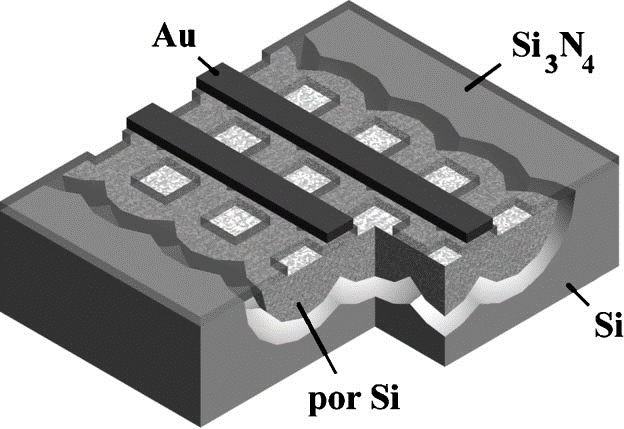
\includegraphics[width=1.\textwidth]{figures/Microspectrometer based on a tunable optical filter of porous silicon_7.png} %插入图片,[]中设置图片大小,{}中是图片文件名
                \caption{电化学刻蚀处理机械臂截面} %最终文档中希望显示的图片标题
            \end{figure}
        \end{column}
    \end{columns}
\end{frame}

\begin{frame}[c]
    \frametitle{基于多孔硅可调谐光学滤光片的微光谱仪:效果}
    \begin{figure}[!htb] %H为当前位置,!htb为忽略美学标准,htbp为浮动图形
        \centering %图片居中
        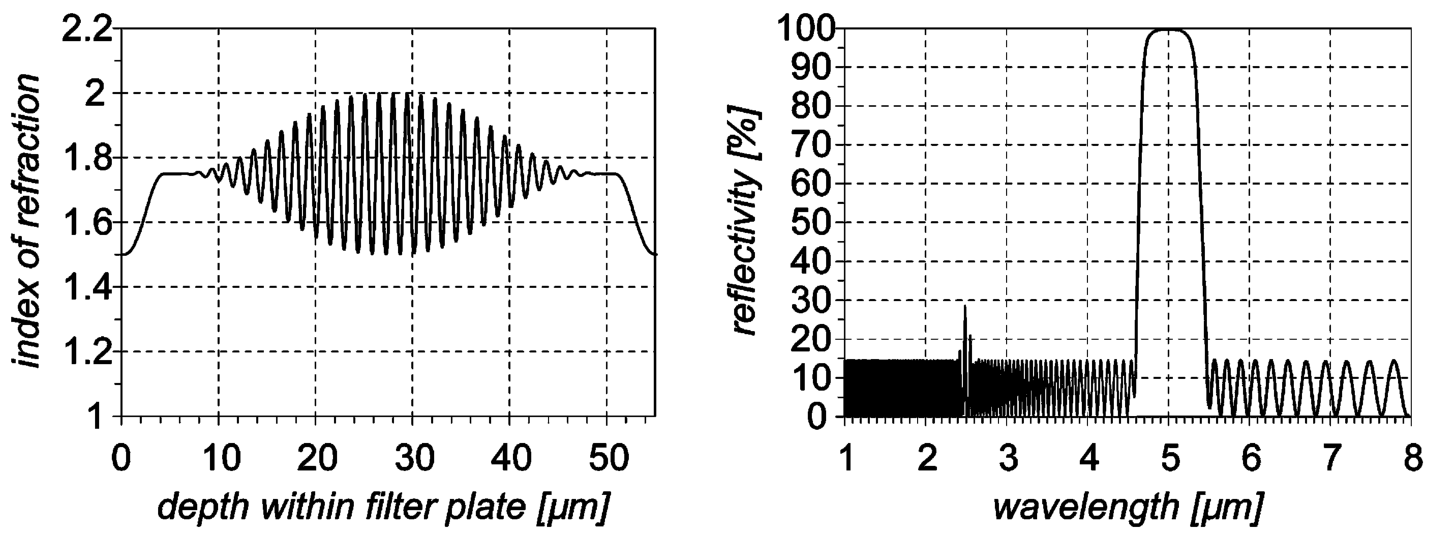
\includegraphics[width=.75\textwidth]{figures/Microspectrometer based on a tunable optical filter of porous silicon_3.png} %插入图片,[]中设置图片大小,{}中是图片文件名
        \caption{可调的折射率和反射镜的反射率} %最终文档中希望显示的图片标题
    \end{figure}
    \begin{itemize}
        \item 通过反射镜的性质可以看到工作波长在 $\lambda=5\ \mathrm{\mu m}$ 左右,范围约 $1\ \mathrm{\mu m}$。
    \end{itemize}

    \begin{columns}
        \begin{column}{.5\textwidth}
            峰值波长关系:\[\lambda_{\theta}=\lambda_0\sqrt{1-(\frac{\sin\theta}{n})^2},\ \lambda_0=2dm\]
        \end{column}
        \begin{column}{.5\textwidth}
            \begin{figure}[!htb] %H为当前位置,!htb为忽略美学标准,htbp为浮动图形
                \centering %图片居中
                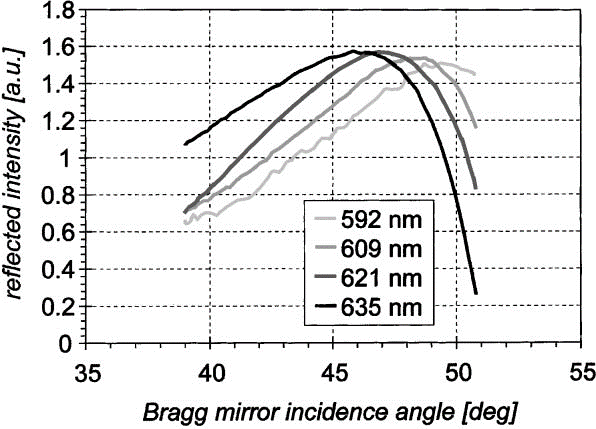
\includegraphics[width=.75\textwidth]{figures/Microspectrometer based on a tunable optical filter of porous silicon_4.png} %插入图片,[]中设置图片大小,{}中是图片文件名
                \caption{峰值波长和角度的关系} %最终文档中希望显示的图片标题
            \end{figure}
        \end{column}
    \end{columns}
\end{frame}